\documentclass{article}
\usepackage[margin=1in]{geometry}
\usepackage[linesnumbered,ruled,vlined]{algorithm2e}
\usepackage{amsfonts}
\usepackage{amsmath}
\usepackage{amssymb}
\usepackage{amsthm}
\usepackage{enumitem}
\usepackage{fancyhdr}
\usepackage{hyperref}
\usepackage{minted}
\usepackage{multicol}
\usepackage{pdfpages}
\usepackage{standalone}
\usepackage[many]{tcolorbox}
\usepackage{tikz-cd}
\usepackage{transparent}
\usepackage{xcolor}
% \tcbuselibrary{minted}

\author{Nathan Solomon}

\newcommand{\fig}[1]{
    \begin{center}
        \includegraphics[width=\textwidth]{#1}
    \end{center}
}

% Math commands
\renewcommand{\d}{\mathrm{d}}
\DeclareMathOperator{\id}{id}
\DeclareMathOperator{\im}{im}
\DeclareMathOperator{\proj}{proj}
\DeclareMathOperator{\Span}{span}
\DeclareMathOperator{\Tr}{Tr}
\DeclareMathOperator{\tr}{tr}
\DeclareMathOperator{\ad}{ad}
\DeclareMathOperator{\ord}{ord}
%%%%%%%%%%%%%%% \DeclareMathOperator{\sgn}{sgn}
\DeclareMathOperator{\Aut}{Aut}
\DeclareMathOperator{\Inn}{Inn}
\DeclareMathOperator{\Out}{Out}
\DeclareMathOperator{\stab}{stab}

\newcommand{\N}{\ensuremath{\mathbb{N}}}
\newcommand{\Z}{\ensuremath{\mathbb{Z}}}
\newcommand{\Q}{\ensuremath{\mathbb{Q}}}
\newcommand{\R}{\ensuremath{\mathbb{R}}}
\newcommand{\C}{\ensuremath{\mathbb{C}}}
\renewcommand{\H}{\ensuremath{\mathbb{H}}}
\newcommand{\F}{\ensuremath{\mathbb{F}}}

\newcommand{\E}{\ensuremath{\mathbb{E}}}
\renewcommand{\P}{\ensuremath{\mathbb{P}}}

\newcommand{\es}{\ensuremath{\varnothing}}
\newcommand{\inv}{\ensuremath{^{-1}}}
\newcommand{\eps}{\ensuremath{\varepsilon}}
\newcommand{\del}{\ensuremath{\partial}}
\renewcommand{\a}{\ensuremath{\alpha}}

\newcommand{\abs}[1]{\ensuremath{\left\lvert #1 \right\rvert}}
\newcommand{\norm}[1]{\ensuremath{\left\lVert #1\right\rVert}}
\newcommand{\mean}[1]{\ensuremath{\left\langle #1 \right\rangle}}
\newcommand{\floor}[1]{\ensuremath{\left\lfloor #1 \right\rfloor}}
\newcommand{\ceil}[1]{\ensuremath{\left\lceil #1 \right\rceil}}
\newcommand{\bra}[1]{\ensuremath{\left\langle #1 \right\rvert}}
\newcommand{\ket}[1]{\ensuremath{\left\lvert #1 \right\rangle}}
\newcommand{\braket}[2]{\ensuremath{\left.\left\langle #1\right\vert #2 \right\rangle}}

\newcommand{\catname}[1]{{\normalfont\textbf{#1}}}

\newcommand{\up}{\ensuremath{\uparrow}}
\newcommand{\down}{\ensuremath{\downarrow}}

% Custom environments
\newtheorem{thm}{Theorem}[section]

\definecolor{probBackgroundColor}{RGB}{250,240,240}
\definecolor{probAccentColor}{RGB}{140,40,0}
\newenvironment{prob}{
    \stepcounter{thm}
    \begin{tcolorbox}[
        boxrule=1pt,
        sharp corners,
        colback=probBackgroundColor,
        colframe=probAccentColor,
        borderline west={4pt}{0pt}{probAccentColor},
        breakable
    ]
    \color{probAccentColor}\textbf{Problem \thethm.} \color{black}
} {
    \end{tcolorbox}
}

\definecolor{exampleBackgroundColor}{RGB}{212,232,246}
\newenvironment{example}{
    \stepcounter{thm}
    \begin{tcolorbox}[
      boxrule=1pt,
      sharp corners,
      colback=exampleBackgroundColor,
      breakable
    ]
    \textbf{Example \thethm.}
} {
    \end{tcolorbox}
}

\definecolor{propBackgroundColor}{RGB}{255,245,220}
\definecolor{propAccentColor}{RGB}{150,100,0}
\newenvironment{prop}{
    \stepcounter{thm}
    \begin{tcolorbox}[
        boxrule=1pt,
        sharp corners,
        colback=propBackgroundColor,
        colframe=propAccentColor,
        breakable
    ]
    \color{propAccentColor}\textbf{Proposition \thethm. }\color{black}
} {
    \end{tcolorbox}
}

\definecolor{thmBackgroundColor}{RGB}{235,225,245}
\definecolor{thmAccentColor}{RGB}{50,0,100}
\renewenvironment{thm}{
    \stepcounter{thm}
    \begin{tcolorbox}[
        boxrule=1pt,
        sharp corners,
        colback=thmBackgroundColor,
        colframe=thmAccentColor,
        breakable
    ]
    \color{thmAccentColor}\textbf{Theorem \thethm. }\color{black}
} {
    \end{tcolorbox}
}

\definecolor{corBackgroundColor}{RGB}{240,250,250}
\definecolor{corAccentColor}{RGB}{50,100,100}
\newenvironment{cor}{
    \stepcounter{thm}
    \begin{tcolorbox}[
        enhanced,
        boxrule=0pt,
        frame hidden,
        sharp corners,
        colback=corBackgroundColor,
        borderline west={4pt}{0pt}{corAccentColor},
        breakable
    ]
    \color{corAccentColor}\textbf{Corollary \thethm. }\color{black}
} {
    \end{tcolorbox}
}

\definecolor{lemBackgroundColor}{RGB}{255,245,235}
\definecolor{lemAccentColor}{RGB}{250,125,0}
\newenvironment{lem}{
    \stepcounter{thm}
    \begin{tcolorbox}[
        enhanced,
        boxrule=0pt,
        frame hidden,
        sharp corners,
        colback=lemBackgroundColor,
        borderline west={4pt}{0pt}{lemAccentColor},
        breakable
    ]
    \color{lemAccentColor}\textbf{Lemma \thethm. }\color{black}
} {
    \end{tcolorbox}
}

\definecolor{proofBackgroundColor}{RGB}{255,255,255}
\definecolor{proofAccentColor}{RGB}{80,80,80}
\renewenvironment{proof}{
    \begin{tcolorbox}[
        enhanced,
        boxrule=1pt,
        sharp corners,
        colback=proofBackgroundColor,
        colframe=proofAccentColor,
        borderline west={4pt}{0pt}{proofAccentColor},
        breakable
    ]
    \color{proofAccentColor}\emph{\textbf{Proof. }}\color{black}
} {
    \qed \end{tcolorbox}
}

\definecolor{noteBackgroundColor}{RGB}{240,250,240}
\definecolor{noteAccentColor}{RGB}{30,130,30}
\newenvironment{note}{
    \begin{tcolorbox}[
        enhanced,
        boxrule=0pt,
        frame hidden,
        sharp corners,
        colback=noteBackgroundColor,
        borderline west={4pt}{0pt}{noteAccentColor},
        breakable
    ]
    \color{noteAccentColor}\textbf{Note. }\color{black}
} {
    \end{tcolorbox}
}


\fancyhf{}
\setlength{\headheight}{24pt}

\date{\today}
\title{Math 151A Homework \#8}

\begin{document}
\maketitle

\begin{prob}
\end{prob}
\begin{enumerate}[label=(\alph*)]
    \item $x_1=x_2=1$
    \begin{center}
        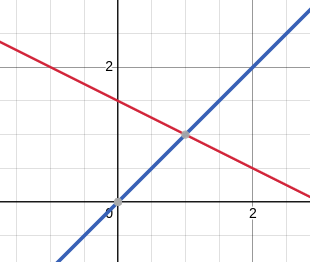
\includegraphics[width=0.5\textwidth]{1a.png}
    \end{center}
\item The red and blue lines completely overlap, so there are infinitely many solutions.
    \begin{center}
        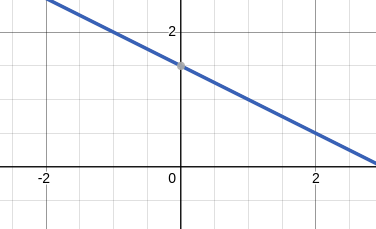
\includegraphics[width=0.5\textwidth]{1b.png}
    \end{center}
\end{enumerate}


\bigskip
\begin{prob}
\end{prob}
\begin{enumerate}[label=(\alph*)]
    \item
    \item
\end{enumerate}


\bigskip
\begin{prob}
\end{prob}
Let
        \[ A := \begin{bmatrix}
            2 & -6\alpha \\
            3\alpha & -1
        \end{bmatrix}. \]
The determinant of this matrix is
        \[ \det(A) = (2)(-1)-(-6\alpha)(3\alpha)=18\alpha^2-2. \]
Therefore $A$ is singular iff $\alpha=\pm 1/3$. The equation
\[ A \begin{bmatrix}
    x_1 \\
    x_2
\end{bmatrix} = \begin{bmatrix}
    3 \\
    3/2
\end{bmatrix} \]
has exactly one solution if $A$ is nonsingular, so we just need to test two possible values of $\alpha$. If $\alpha=1/3$, the system of equations is equivalent to
\begin{align*}
    2 x_1 - 2 x_2 &= 3 \\
    x_1 - x_2 = 3/2,
\end{align*}
which has infinitely many solutions because for any $x_1 \in \R$, $x_2=x_1-3/2$ is a solution. If $\alpha=-1/3$, the system of equations is
\begin{align*}
    2 x_1 + 2 x_2 &= 3 \\
    -x_1 - x_2 = 3/2,
\end{align*}
which has no solutions, because doubling the second equation and adding it to the first gives $0=6$, which is never true.
\par
If $\alpha \not\in \left\{ -1/3,1/3 \right\}$, then
\[ \begin{bmatrix}
    x_1 \\
    x_2
\end{bmatrix} = A^{-1} \begin{bmatrix}
    3 \\
    3/2
    \end{bmatrix} = \frac{1}{\det(A)} \begin{bmatrix}
    -1 & 3\alpha \\
    -6\alpha & 2
\end{bmatrix} \begin{bmatrix}
    3 \\
    3/2
\end{bmatrix} = \frac{1}{18\alpha^2-2} \begin{bmatrix}
    4.5\alpha-3 \\
    3-18\alpha
\end{bmatrix}. \]

\bigskip
\begin{prob}
\end{prob}


\bigskip
\begin{prob}
\end{prob}
By Sarrus' rule,
\begin{align*}
    \det(A) &= (1)(2)(-1.5)+(-1)(1)(0)+(\alpha)(2)(\alpha)-(\alpha)(2)(0)-(-1)(2)(-1.5)-(1)(1)(\alpha) \\
            &= -3+2\alpha^2-3+\alpha \\
            &= \alpha(2\alpha+1).
\end{align*}
So $A$ is singular iff $\alpha \in \left\{ 0, 1/2 \right\}$.

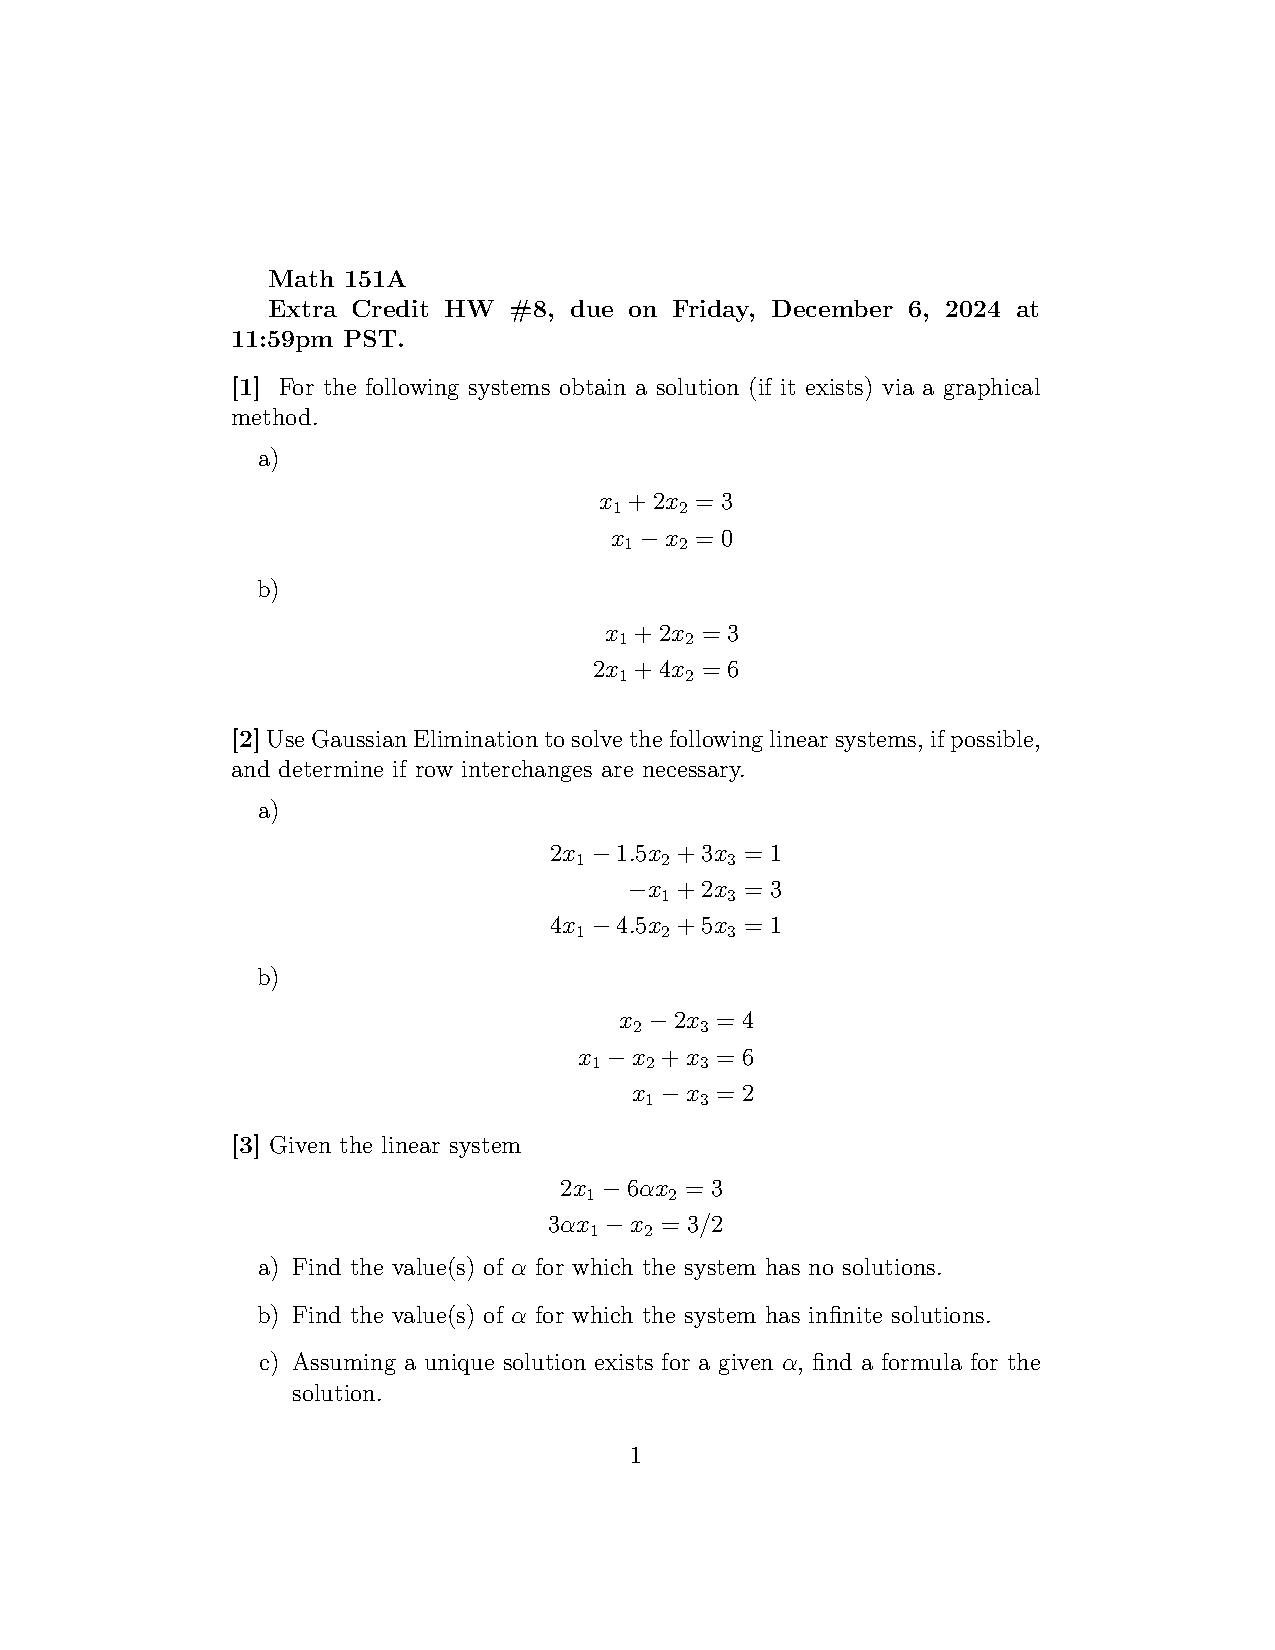
\includepdf[pages=-]{assignment.pdf}

\end{document}
